\documentclass[12pt, twocolumn, a4paper]{article}
% -------------------------------------------------------------------
% Package I use
% -------------------------------------------------------------------
\usepackage{tabularx} % enable us able to make tables
\usepackage{graphicx} % enable us able to include graphs
\usepackage{amsmath} % makes some nice additions to math
\usepackage{amssymb} % gives us mathbb 
% -------------------------------------------------------------------
% Title setup:
\title{The exponential function}
\author{Anders Kragh}
\date{\today}
% -------------------------------------------------------------------
% Begining the document
% ------------------------------------------------------------------- 
\begin{document}
\maketitle
\section{Introduction}
The real exponential function is define as  function, which takes values from $ \mathbb{R} \to \mathbb{R}$. It can be defined by the taylor serie:
\begin{align}
\exp \left( x \right) &= \sum_{i=0}^{\infty}  \frac{x^i}{i!} \label{eq: taylor-serie}\tag{$\star$}
\end{align}
Looking at equation \eqref{eq: taylor-serie} we can conclude that the nummber in the base $\exp \left(x \right) = e^{x}$ is given by
\begin{align}
e  = \exp \left(1 \right) = \sum_{i=0}^{\infty}  \frac{1^i}{i!} = \sum_{i=0}^{\infty}  \frac{1}{i!}. \label{eq: e}
\end{align}
The exponential function is also define for a complex number, where is appears in Euler's formula 
\begin{align}
\exp \left( i\cdot x \right) &= \cos \left(x \right) + i \cdot \sin \left( x \right) \label{eq: euler}
\end{align}
\subsection{Other definition of the expexponential function}
Other way to define the exponential function is as a solution to the differential equation:
\begin{align}
\frac{\text{d}y}{\text{d}x} &= y \label{eq: diff}
\end{align}
with the initial condition of $y\left(0 \right) = 1$.
Another way tp define the exponential function is as a limit when $n$ goes to infinity of
\begin{align}
\exp \left( x \right) &= \lim_{n\to \infty} \left(1+\frac{x}{n}\right)^{n} \label{eq: lim}
\end{align}
\section{Numerical approach to exponential function}
Our "quick-and-dirty" implementation of the exponential function, is taking the have calculated the taylor serie $\left(\text{equation \eqref{eq: taylor-serie}} \right)$ to $n=10$ and uses it for our calculation.
If we receive a negative number, $x$, we will call our function recursive with $\frac{1}{\exp \left(x \right)}$ since $a^{-b} = \frac{1}{a^{b}}$. To make sure our function is precise, we will call the function recursively with $\left( \exp \left( \frac{x}{2} \right) \right)^{2}$ if the function is called with $x$ value greater than $\frac{1}{8}$.
At figure \ref{fig:exp_dirty-approach} we can see the result of our numerical approach to exponential function alongside with the actual values, which can be found in table \ref{tab_exp}
\begin{figure} \label{fig:exp_dirty-approach}
	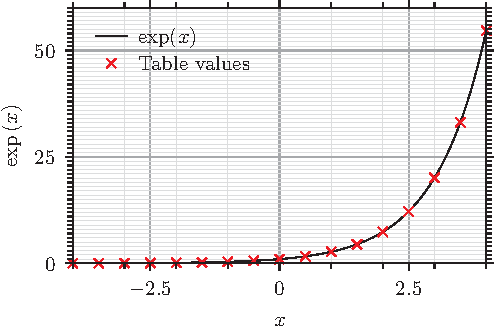
\includegraphics[width=\columnwidth]{exp_pyx.pdf}
	\caption{A plot of the "quick-and-dirty" implementation of the exponential function in the interval $\left[-4, 4\right]$. Alongs with the plots of points of the actual exponential function}
\end{figure}

\begin{table}
	\begin{center}
		\caption{Values of $x$ and $\exp \left( x \right)$ calculated with System.Math.Exp in C\#.}
	    \begin{tabular}{| c | c |}
	    \hline
	    $x$ & $\exp \left(x\right)$ \\ \hline
	    $-4$ & $0.0183156388887342$ \\
		\hline
		$-3.5$ & $0.0301973834223185$\\
		\hline
		$-3$ & $ 0.0497870683678639$ \\ 
		\hline
		$-2.5$ & $ 0.0820849986238988$ \\ 
		\hline
		$-2$ & $ 0.135335283236613$ \\ 
		\hline
		$-1.5$ & $ 0.22313016014843$ \\ 
		\hline
		$-1$ & $ 0.367879441171442$ \\ 
		\hline
		$-0.5$ & $ 0.606530659712633$ \\ 
		\hline
		$0$ & $ 1$ \\ 
		\hline
		$0.5$ & $ 1.64872127070013$ \\ 
		\hline
		$1$ & $ 2.71828182845905$ \\ 
		\hline
		$1.5$ & $ 4.48168907033806$ \\ 
		\hline
		$2$ & $ 7.38905609893065$ \\ 
		\hline
		$2.5$ & $ 12.1824939607035$ \\ 
		\hline
		$3$ & $ 20.0855369231877$ \\ 
		\hline
		$3.5$ & $ 33.1154519586923$ \\ 
		\hline
		$4$ & $ 54.5981500331442$ \\
		\hline
	    \end{tabular}
	\label{tab_exp}
	\end{center}
\end{table}
\section{Evaluation of our numerical approach}
As we see on figure \ref{fig:exp_dirty-approach} our approch is close to the value, and if we use our to calculate our approch to eulers number as
\begin{align}
e_{\text{approach}} &= \sum_{i=0}^{10} \frac{1}{i!} \nonumber\\
&\approx 2.71828180 \label{eq: e_dirty}
\end{align}
Comparing equation \eqref{eq: e_dirty} to our tabel value of $\exp\left(1\right)$ from table \ref{tab_exp} is on the $8^{\text{th}}$ decimal our approach begins to vary from eulers number in equation \eqref{eq: e}.
\end{document}